%%%%%%%%%%%%%%%%%%%%%%%%%%%%%%%%%%%%%%%%%
%
% Important note:
% Chapter heading images should have a 2:1 width:height ratio,
% e.g. 920px width and 460px height.
%
% The original template (the Legrand Orange Book Template) can be found here --> http://www.latextemplates.com/template/the-legrand-orange-book
%
% Original author of the Legrand Orange Book Template:
% Mathias Legrand (legrand.mathias@gmail.com) with modifications by: Vel (vel@latextemplates.com)
%
% Original License:
% CC BY-NC-SA 3.0 (http://creativecommons.org/licenses/by-nc-sa/3.0/)
%%%%%%%%%%%%%%%%%%%%%%%%%%%%%%%%%%%%%%%%%


%----------------------------------------------------------------------------------------
%	CETNTRAL VARIABLES
%----------------------------------------------------------------------------------------
\def\meinTitel{Sicherheit von KI-Systemen in Luftfahrtradarsystemen}
\def\TODO{\textcolor{Red}{TODO}}

\newcommand{\scriptTitle}{\meinTitel}
\newcommand{\scriptAuthor}{Tomy Hebel 78280}
\newcommand{\scriptSubject}{\meinTitel}
\newcommand{\scriptKeywords}{25sose\_Bachelor\_Thesis}
\newcommand{\scriptFaculty}{Maschinenbau und Mechatronik}
\newcommand{\scriptCourse}{Bachelor Thesis Sommersemester 2025}
\newcommand{\scriptPublisher}{Tomy Hebel}
\newcommand{\scriptWebsite}{https://ilias.h-ka.de}
\newcommand{\scriptLicense}{CC BY-NC-SA 3.0 (http://creativecommons.org/licenses/by-nc-sa/3.0/)}
\newcommand{\scriptEdition}{Erste Ausgabe, Stand: April 2025}

%----------------------------------------------------------------------------------------
%	PACKAGES AND OTHER DOCUMENT CONFIGURATIONS
%----------------------------------------------------------------------------------------

\documentclass[11pt,fleqn, oneside]{book} % Default font size and left-justified equations

%%%%%%%%%%%%%%%%%%%%%%%%%%%%%%%%%%%%%%%%%
% The Legrand Orange Book
% Structural Definitions File
% Version 2.1 (26/09/2018)
%
% Original author:
% Mathias Legrand (legrand.mathias@gmail.com) with modifications by:
% Vel (vel@latextemplates.com)
% 
% This file was downloaded from:
% http://www.LaTeXTemplates.com
%
% License:
% CC BY-NC-SA 3.0 (http://creativecommons.org/licenses/by-nc-sa/3.0/)
%
%%%%%%%%%%%%%%%%%%%%%%%%%%%%%%%%%%%%%%%%%

%	Abkürzungen
\usepackage{acronym}

%----------------------------------------------------------------------------------------
%	MARGINS
%----------------------------------------------------------------------------------------

\usepackage{geometry} % Required for adjusting page dimensions and margins

\geometry{
	paper=a4paper, % Paper size, change to letterpaper for US letter size
	top=3cm, % Top margin
	bottom=3cm, % Bottom margin
	left=3cm, % Left margin
	right=3cm, % Right margin
	headheight=14pt, % Header height
	footskip=1.4cm, % Space from the bottom margin to the baseline of the footer
	headsep=10pt, % Space from the top margin to the baseline of the header
	%showframe, % Uncomment to show how the type block is set on the page
}

\setlength{\parindent}{0pt} % Kein Einzug für die erste Zeile jedes Absatzes

%----------------------------------------------------------------------------------------
%	FONTS
%----------------------------------------------------------------------------------------
\usepackage[T1]{fontenc} % Ensures proper hyphenation of special characters
\usepackage[utf8]{inputenc} % Allows use of accented characters
\usepackage[ngerman]{babel} % German language support
\usepackage{csquotes} % Correct quotation marks in the respective language

\usepackage{avant} % Use the Avantgarde font for headings
\newcommand*{\avantstyle}{\fontfamily{pag}\selectfont}
\DeclareTextFontCommand{\avantfont}{\avantstyle}

\usepackage{plex-sans}

\renewcommand*\familydefault{\sfdefault} %% Only if the base font of the document is to be sans serif
%\usepackage{mathptmx} % Use the Adobe Times Roman as the default text font together with math symbols from the Sym­bol, Chancery and Com­puter Modern fonts

\usepackage{microtype} % Slightly tweak font spacing for aesthetics

%----------------------------------------------------------------------------------------
%	BIBLIOGRAPHY AND INDEX
%----------------------------------------------------------------------------------------

\usepackage[style=numeric,citestyle=numeric,sorting=nyt,sortcites=true,autopunct=true,hyperref=true,abbreviate=false,backref=true,backend=biber]{biblatex}
\addbibresource{bibliography.bib} % BibTeX bibliography file
\defbibheading{bibempty}{}

\usepackage{calc} % For simpler calculation - used for spacing the index letter headings correctly
\usepackage{makeidx} % Required to make an index
\makeindex % Tells LaTeX to create the files required for indexing

%----------------------------------------------------------------------------------------
%	DIGITAL LOGIC & ELECTRONICS
%----------------------------------------------------------------------------------------

\usepackage[european, RPvoltages]{circuitikz}

%----------------------------------------------------------------------------------------
%	MAIN TABLE OF CONTENTS
%----------------------------------------------------------------------------------------

\usepackage{titletoc} % Required for manipulating the table of contents

\contentsmargin{0cm} % Removes the default margin

% Part text styling (this is mostly taken care of in the PART HEADINGS section of this file)
\titlecontents{part}
	[0cm] % Left indentation
	{\addvspace{20pt}\bfseries} % Spacing and font options for parts
	{}
	{}
	{}

% Chapter text styling
\titlecontents{chapter}
	[1.25cm] % Left indentation
	{\addvspace{12pt}\large\sffamily\bfseries} % Spacing and font options for chapters
	{\color{ThemeColor}\contentslabel[\Large\thecontentslabel]{1.25cm}\color{ThemeColor}} % Formatting of numbered sections of this type
	{\color{ThemeColor}} % Formatting of numberless sections of this type
	{\color{ThemeColor}\normalsize\;\titlerule*[.5pc]{.}\;\thecontentspage} % Formatting of the filler to the right of the heading and the page number

% Section text styling
\titlecontents{section}
	[1.25cm] % Left indentation
	{\addvspace{3pt}\sffamily\bfseries} % Spacing and font options for sections
	{\contentslabel[\thecontentslabel]{1.25cm}} % Formatting of numbered sections of this type
	{} % Formatting of numberless sections of this type
	{\hfill\color{black}\thecontentspage} % Formatting of the filler to the right of the heading and the page number

% Subsection text styling
\titlecontents{subsection}
	[1.25cm] % Left indentation
	{\addvspace{1pt}\sffamily\small} % Spacing and font options for subsections
	{\contentslabel[\thecontentslabel]{1.25cm}} % Formatting of numbered sections of this type
	{} % Formatting of numberless sections of this type
	{\ \titlerule*[.5pc]{.}\;\thecontentspage} % Formatting of the filler to the right of the heading and the page number

% Figure text styling
\titlecontents{figure}
	[1.25cm] % Left indentation
	{\addvspace{1pt}\sffamily\small} % Spacing and font options for figures
	{\thecontentslabel\hspace*{1em}} % Formatting of numbered sections of this type
	{} % Formatting of numberless sections of this type
	{\ \titlerule*[.5pc]{.}\;\thecontentspage} % Formatting of the filler to the right of the heading and the page number

% Table text styling
\titlecontents{table}
	[1.25cm] % Left indentation
	{\addvspace{1pt}\sffamily\small} % Spacing and font options for tables
	{\thecontentslabel\hspace*{1em}} % Formatting of numbered sections of this type
	{} % Formatting of numberless sections of this type
	{\ \titlerule*[.5pc]{.}\;\thecontentspage} % Formatting of the filler to the right of the heading and the page number

%----------------------------------------------------------------------------------------
%	MINI TABLE OF CONTENTS IN PART HEADS
%----------------------------------------------------------------------------------------

% To override the existing colorred text
\newcommand{\absolutetextcolor}[2]{%
    \textcolor{#1}{%
        \renewcommand\textcolor[2][]{}%
    #2}%
}

% Chapter text styling
\titlecontents{lchapter}
	[0em] % Left indentation
	{\addvspace{15pt}\large\sffamily\bfseries} % Spacing and font options for chapters
	{\color{white}\contentslabel[\Large\thecontentslabel]{1.25cm}\color{white}} % Chapter number
	{\absolutetextcolor{white}}
	{\color{white}\normalsize\sffamily\bfseries\;\titlerule*[.5pc]{.}\;\thecontentspage} % Page number

% Section text styling
\titlecontents{lsection}
	[0em] % Left indentation
	{\color{white}\sffamily\small} % Spacing and font options for sections
	{\contentslabel[\thecontentslabel]{1.25cm}} % Section number
	{}
	{}

% Subsection text styling (note these aren't shown by default, display them by searchings this file for tocdepth and reading the commented text)
\titlecontents{lsubsection}
	[.5em] % Left indentation
	{\color{white}\sffamily\footnotesize} % Spacing and font options for subsections
	{\contentslabel[\thecontentslabel]{1.25cm}}
	{}
	{}

%----------------------------------------------------------------------------------------
%	HEADERS AND FOOTERS
%----------------------------------------------------------------------------------------

\usepackage{fancyhdr} % Required for header and footer configuration

\pagestyle{fancy} % Enable the custom headers and footers

\renewcommand{\chaptermark}[1]{\markboth{\sffamily\normalsize\bfseries\chaptername\ \thechapter.\ #1}{}} % Styling for the current chapter in the header
\renewcommand{\sectionmark}[1]{\markright{\sffamily\normalsize\thesection\hspace{5pt}#1}{}} % Styling for the current section in the header

\fancyhf{} % Clear default headers and footers
\fancyhead[LE,RO]{\sffamily\normalsize\thepage} % Styling for the page number in the header
\fancyhead[LO]{\rightmark} % Print the nearest section name on the left side of odd pages
\fancyhead[RE]{\leftmark} % Print the current chapter name on the right side of even pages
%\fancyfoot[C]{\thepage} % Uncomment to include a footer

\renewcommand{\headrulewidth}{0.5pt} % Thickness of the rule under the header

\fancypagestyle{plain}{% Style for when a plain pagestyle is specified
	\fancyhead{}\renewcommand{\headrulewidth}{0pt}%
}

% Removes the header from odd empty pages at the end of chapters
\makeatletter	% Einkommentieren für leeere Seiten /page /newpage /ungerade seiten zahlen
%\renewcommand{\cleardoublepage}{
%\clearpage\ifodd\c@page\else
%\hbox{}
%\vspace*{\fill}
%\thispagestyle{empty}
%\newpage
%\fi}

%----------------------------------------------------------------------------------------
%	THEOREM STYLES
%----------------------------------------------------------------------------------------

\usepackage{amsmath,amsfonts,amssymb,amsthm} % For math equations, theorems, symbols, etc

\newcommand{\intoo}[2]{\mathopen{]}#1\,;#2\mathclose{[}}
\newcommand{\ud}{\mathop{\mathrm{{}d}}\mathopen{}}
\newcommand{\intff}[2]{\mathopen{[}#1\,;#2\mathclose{]}}
\renewcommand{\qedsymbol}{$\blacksquare$}
\newtheorem{notation}{Notation}[chapter]

% Boxed/framed environments
\newtheoremstyle{ThemeColornumbox}% Theorem style name
{0pt}% Space above
{0pt}% Space below
{\normalfont}% Body font
{}% Indent amount
{\small\bf\sffamily\color{ThemeColor}}% Theorem head font
{\;}% Punctuation after theorem head
{0.25em}% Space after theorem head
{\small\sffamily\color{ThemeColor}\thmname{#1}\nobreakspace\thmnumber{\@ifnotempty{#1}{}\@upn{#2}}% Theorem text (e.g. Theorem 2.1)
\thmnote{\nobreakspace\the\thm@notefont\sffamily\bfseries\color{black}---\nobreakspace#3.}} % Optional theorem note

\newtheoremstyle{blacknumex}% Theorem style name
{5pt}% Space above
{5pt}% Space below
{\normalfont}% Body font
{} % Indent amount
{\small\bf\sffamily}% Theorem head font
{\;}% Punctuation after theorem head
{0.25em}% Space after theorem head
{\small\sffamily{\tiny\ensuremath{\blacksquare}}\nobreakspace\thmname{#1}\nobreakspace\thmnumber{\@ifnotempty{#1}{}\@upn{#2}}% Theorem text (e.g. Theorem 2.1)
\thmnote{\nobreakspace\the\thm@notefont\sffamily\bfseries---\nobreakspace#3.}}% Optional theorem note

\newtheoremstyle{blacknumbox} % Theorem style name
{0pt}% Space above
{0pt}% Space below
{\normalfont}% Body font
{}% Indent amount
{\small\bf\sffamily}% Theorem head font
{\;}% Punctuation after theorem head
{0.25em}% Space after theorem head
{\small\sffamily\thmname{#1}\nobreakspace\thmnumber{\@ifnotempty{#1}{}\@upn{#2}}% Theorem text (e.g. Theorem 2.1)
\thmnote{\nobreakspace\the\thm@notefont\sffamily\bfseries---\nobreakspace#3.}}% Optional theorem note

% Non-boxed/non-framed environments
\newtheoremstyle{ThemeColornum}% Theorem style name
{5pt}% Space above
{5pt}% Space below
{\normalfont}% Body font
{}% Indent amount
{\small\bf\sffamily\color{ThemeColor}}% Theorem head font
{\;}% Punctuation after theorem head
{0.25em}% Space after theorem head
{\small\sffamily\color{ThemeColor}\thmname{#1}\nobreakspace\thmnumber{\@ifnotempty{#1}{}\@upn{#2}}% Theorem text (e.g. Theorem 2.1)
\thmnote{\nobreakspace\the\thm@notefont\sffamily\bfseries\color{black}---\nobreakspace#3.}} % Optional theorem note
\makeatother

% Defines the theorem text style for each type of theorem to one of the three styles above
%\newcounter{dummy} 
%\numberwithin{dummy}{section}
%\theoremstyle{ThemeColornumbox}
%\newtheorem{theoremeT}[dummy]{Theorem}
%\newtheorem{problem}{Problem}[chapter]
%\newtheorem{exerciseT}{Exercise}[chapter]
%\theoremstyle{blacknumex}
%\newtheorem{exampleT}{Example}[chapter]
%\theoremstyle{blacknumbox}
%\newtheorem{vocabulary}{Vocabulary}[chapter]
%\newtheorem{definitionT}{Definition}[section]
%\newtheorem{corollaryT}[dummy]{Corollary}
%\theoremstyle{ThemeColornum}
%\newtheorem{proposition}[dummy]{Proposition}

% Deutsche Begriffe fuer Theorem-Boxen
\newcounter{dummy} 
\numberwithin{dummy}{section}
\theoremstyle{ThemeColornumbox}
\newtheorem{theoremeT}[dummy]{Satz}
\newtheorem{problem}{Problem}[chapter]
\newtheorem{exerciseT}{\"Ubung}[chapter]
\theoremstyle{blacknumex}
\newtheorem{exampleT}{Beispiel}[chapter]
\theoremstyle{blacknumbox}
\newtheorem{vocabulary}{W\"orterverzeichnis }[chapter]
\newtheorem{definitionT}{Definition}[section]
\newtheorem{corollaryT}[dummy]{Folgerung}
\theoremstyle{ThemeColornum}
\newtheorem{proposition}[dummy]{These}


%----------------------------------------------------------------------------------------
%	DEFINITION OF COLORED BOXES
%----------------------------------------------------------------------------------------

\RequirePackage[framemethod=default]{mdframed} % Required for creating the theorem, definition, exercise and corollary boxes

% Theorem box
\newmdenv[skipabove=7pt,
skipbelow=7pt,
backgroundcolor=black!5,
linecolor=ThemeColor,
innerleftmargin=5pt,
innerrightmargin=5pt,
innertopmargin=5pt,
leftmargin=0cm,
rightmargin=0cm,
innerbottommargin=5pt]{tBox}

% Exercise box	  
\newmdenv[skipabove=7pt,
skipbelow=7pt,
rightline=false,
leftline=true,
topline=false,
bottomline=false,
backgroundcolor=ThemeColor!10,
linecolor=ThemeColor,
innerleftmargin=5pt,
innerrightmargin=5pt,
innertopmargin=5pt,
innerbottommargin=5pt,
leftmargin=0cm,
rightmargin=0cm,
linewidth=4pt]{eBox}	

% Definition box
\newmdenv[skipabove=7pt,
skipbelow=7pt,
rightline=false,
leftline=true,
topline=false,
bottomline=false,
linecolor=ThemeColor,
innerleftmargin=5pt,
innerrightmargin=5pt,
innertopmargin=0pt,
leftmargin=0cm,
rightmargin=0cm,
linewidth=4pt,
innerbottommargin=0pt]{dBox}	

% Corollary box
\newmdenv[skipabove=7pt,
skipbelow=7pt,
rightline=false,
leftline=true,
topline=false,
bottomline=false,
linecolor=gray,
backgroundcolor=black!5,
innerleftmargin=5pt,
innerrightmargin=5pt,
innertopmargin=5pt,
leftmargin=0cm,
rightmargin=0cm,
linewidth=4pt,
innerbottommargin=5pt]{cBox}

% Creates an environment for each type of theorem and assigns it a theorem text style from the "Theorem Styles" section above and a colored box from above
\newenvironment{theorem}{\begin{tBox}\begin{theoremeT}}{\end{theoremeT}\end{tBox}}
\newenvironment{exercise}{\begin{eBox}\begin{exerciseT}}{\hfill{\color{ThemeColor}\tiny\ensuremath{\blacksquare}}\end{exerciseT}\end{eBox}}				  
\newenvironment{definition}{\begin{dBox}\begin{definitionT}}{\end{definitionT}\end{dBox}}	
\newenvironment{example}{\begin{exampleT}}{\hfill{\tiny\ensuremath{\blacksquare}}\end{exampleT}}		
\newenvironment{corollary}{\begin{cBox}\begin{corollaryT}}{\end{corollaryT}\end{cBox}}	

%----------------------------------------------------------------------------------------
%	REMARK ENVIRONMENT
%----------------------------------------------------------------------------------------

\newenvironment{remark}{\par\vspace{10pt}\small % Vertical white space above the remark and smaller font size
\begin{list}{}{
\leftmargin=35pt % Indentation on the left
\rightmargin=25pt}\item\ignorespaces % Indentation on the right
\makebox[-2.5pt]{\begin{tikzpicture}[overlay]
\node[draw=ThemeColor,line width=1pt,circle,fill=ThemeColor!25,font=\sffamily\bfseries,inner sep=2pt,outer sep=0pt] at (-15pt,0pt){\textcolor{ThemeColor}{R}};\end{tikzpicture}} % Orange R in a circle
\advance\baselineskip -1pt}{\end{list}\vskip5pt} % Tighter line spacing and white space after remark

%----------------------------------------------------------------------------------------
%	SECTION NUMBERING IN THE MARGIN
%----------------------------------------------------------------------------------------

\makeatletter
\renewcommand{\@seccntformat}[1]{\llap{\textcolor{ThemeColor}{\csname the#1\endcsname}\hspace{1em}}}                    
\renewcommand{\section}{\@startsection{section}{1}{\z@}
{-4ex \@plus -1ex \@minus -.4ex}
{1ex \@plus.2ex }
{\normalfont\large\sffamily\bfseries}}
\renewcommand{\subsection}{\@startsection {subsection}{2}{\z@}
{-3ex \@plus -0.1ex \@minus -.4ex}
{0.5ex \@plus.2ex }
{\normalfont\sffamily\bfseries}}
\renewcommand{\subsubsection}{\@startsection {subsubsection}{3}{\z@}
{-2ex \@plus -0.1ex \@minus -.2ex}
{.2ex \@plus.2ex }
{\normalfont\small\sffamily\bfseries}}                        
\renewcommand\paragraph{\@startsection{paragraph}{4}{\z@}
{-2ex \@plus-.2ex \@minus .2ex}
{.1ex}
{\normalfont\small\sffamily\bfseries}}

%----------------------------------------------------------------------------------------
%	PART HEADINGS
%----------------------------------------------------------------------------------------

% Numbered part in the table of contents
\newcommand{\@mypartnumtocformat}[2]{%
	\setlength\fboxsep{0pt}%
	\noindent\colorbox{ThemeColor}{\strut\parbox[c][.7cm]{\ecart}{\color{white}\Large\sffamily\bfseries\centering#1}}\hskip\esp\colorbox{ThemeColor}{\strut\parbox[c][.7cm]{\linewidth-\ecart-\esp}{\color{white}\Large\sffamily\centering#2}}%
}

% Unnumbered part in the table of contents
\newcommand{\@myparttocformat}[1]{%
	\setlength\fboxsep{0pt}%
	\noindent\colorbox{ThemeColor}{\strut\parbox[c][.7cm]{\linewidth}{\Large\sffamily\centering#1}}%
}

\newlength\esp
\setlength\esp{4pt}
\newlength\ecart
\setlength\ecart{1.2cm-\esp}
\newcommand{\thepartimage}{}%
\newcommand{\partimage}[1]{\renewcommand{\thepartimage}{#1}}%
\def\@part[#1]#2{%
\ifnum \c@secnumdepth >-2\relax%
\refstepcounter{part}%
\addcontentsline{toc}{part}{\texorpdfstring{\protect\@mypartnumtocformat{\thepart}{#1}}{\partname~\thepart\ ---\ #1}}
\else%
\addcontentsline{toc}{part}{\texorpdfstring{\protect\@myparttocformat{#1}}{#1}}%
\fi%
\startcontents%
\markboth{}{}%
{\thispagestyle{empty}%
\begin{tikzpicture}[remember picture,overlay]%
\node at (current page.north west){\begin{tikzpicture}[remember picture,overlay]%	
\fill[ThemeColor](0cm,0cm) rectangle (\paperwidth,-\paperheight);
\node[anchor=north] at (5.5cm,-3.25cm){\color{white}\fontsize{220}{100}\sffamily\bfseries\thepart}; 
\node[anchor=south east] at (\paperwidth-1cm,-\paperheight+1cm){\parbox[t][][t]{8.5cm}{
\printcontents{l}{0}{\setcounter{tocdepth}{1}}% The depth to which the Part mini table of contents displays headings; 0 for chapters only, 1 for chapters and sections and 2 for chapters, sections and subsections
}};
\node[anchor=north east] at (\paperwidth-1.5cm,-3.25cm){\parbox[t][][t]{8cm}{\strut\raggedleft\color{white}\fontsize{30}{30}\sffamily\bfseries#2}};
\end{tikzpicture}};
\end{tikzpicture}}%
\@endpart}
\def\@spart#1{%
\startcontents%
\phantomsection
{\thispagestyle{empty}%
\begin{tikzpicture}[remember picture,overlay]%
\node at (current page.north west){\begin{tikzpicture}[remember picture,overlay]%	
\fill[ThemeColor!20](0cm,0cm) rectangle (\paperwidth,-\paperheight);
\node[anchor=north east] at (\paperwidth-1.5cm,-3.25cm){\parbox[t][][t]{15cm}{\strut\raggedleft\color{white}\fontsize{30}{30}\sffamily\bfseries#1}};
\end{tikzpicture}};
\end{tikzpicture}}
\addcontentsline{toc}{part}{\texorpdfstring{%
\setlength\fboxsep{0pt}%
\noindent\protect\colorbox{ThemeColor!40}{\strut\protect\parbox[c][.7cm]{\linewidth}{\Large\sffamily\protect\centering #1\quad\mbox{}}}}{#1}}%
\@endpart}
\def\@endpart{\vfil\newpage
\if@twoside
\if@openright
\null
\thispagestyle{empty}%
\newpage
\fi
\fi
\if@tempswa
\twocolumn
\fi}

%----------------------------------------------------------------------------------------
%	CHAPTER HEADINGS
%----------------------------------------------------------------------------------------

% A switch to conditionally include a picture, implemented by Christian Hupfer
\newif\ifusechapterimage
\usechapterimagetrue
\newcommand{\thechapterimage}{}%
\newcommand{\chapterimage}[1]{\ifusechapterimage\renewcommand{\thechapterimage}{#1}\fi}%
\newcommand{\autodot}{.}
\def\@makechapterhead#1{%
	{\parindent \z@ \raggedright \normalfont
		\ifnum \c@secnumdepth >\m@ne

		\if@mainmatter %checks, if chapter is part of mainmatter (no appendix/other)
        \begin{tikzpicture}[remember picture,overlay]
			\node at (current page.north west)
			{\begin{tikzpicture}[remember picture,overlay]
					\node[anchor=north west,inner sep=0pt] at (0,0) {\ifusechapterimage\includegraphics[width=\paperwidth]{\thechapterimage}\fi};

                    %conditionally set position of title
                    \ifusechapterimage
					\draw[anchor=west] (\Gm@lmargin-0cm,-9cm) node [minimum height=2cm, line width=0pt,rounded corners=0pt,draw=white,fill=white,fill opacity=1,inner sep=10pt] {\huge\bfseries\color{ThemeColor}\thechapter\autodot ~#1 \strut};
					\draw[anchor=east] (\Gm@lmargin-0cm,-9cm) node [minimum width=1cm, minimum height=2cm, line width=0pt,rounded corners=0pt, draw=ThemeColor,fill=ThemeColor,fill opacity=1] {};

                    \else
                    \draw[anchor=west] (\Gm@lmargin-0cm,-3cm) node [minimum height=2cm, line width=0pt,rounded corners=0pt,draw=white,fill=white,fill opacity=1,inner sep=10pt] {\huge\bfseries\color{ThemeColor}\thechapter\autodot ~#1 \strut};
					\draw[anchor=east] (\Gm@lmargin-0cm,-3cm) node [minimum width=1cm, minimum height=2cm, line width=0pt,rounded corners=0pt, draw=ThemeColor,fill=ThemeColor,fill opacity=1] {};
                    \fi

			\end{tikzpicture}};
		\end{tikzpicture}

		\else  %draw title for unnumbered chapters --> not @mainmatter
		\begin{tikzpicture}[remember picture,overlay]
			\node at (current page.north west)
			{\begin{tikzpicture}[remember picture,overlay]
					\node[anchor=north west,inner sep=0pt] at (0,0) {\ifusechapterimage\includegraphics[width=\paperwidth]{\thechapterimage}\fi};
     
					\ifusechapterimage
                    \draw[anchor=west] (\Gm@lmargin-0cm,-9cm) node [minimum height=2cm, line width=0pt,rounded corners=0pt,draw=white,fill=white,fill opacity=1,inner sep=10pt] {\huge\bfseries\color{ThemeColor} #1 \strut};
					\draw[anchor=east] (\Gm@lmargin-0cm,-9cm) node [minimum width=1cm, minimum height=2cm, line width=0pt,rounded corners=0pt,draw=ThemeColor,fill=ThemeColor,fill opacity=1] {};
     
                    \else
                    \draw[anchor=west] (\Gm@lmargin-0cm,-3cm) node [minimum height=2cm, line width=0pt,rounded corners=0pt,draw=white,fill=white,fill opacity=1,inner sep=10pt] {\huge\bfseries\color{ThemeColor} #1 \strut};
					\draw[anchor=east] (\Gm@lmargin-0cm,-3cm) node [minimum width=1cm, minimum height=2cm, line width=0pt,rounded corners=0pt,draw=ThemeColor,fill=ThemeColor,fill opacity=1] {};
                    \fi
     
			\end{tikzpicture}};
		\end{tikzpicture}
  
		\fi\fi\par

        \ifusechapterimage
        \vspace*{250\p@}
        \else
        \vspace*{50\p@}
        \fi   
    }}

\def\@makeschapterhead#1{ %make chapterheads for appendix 
	\begin{tikzpicture}[remember picture,overlay]
		\node at (current page.north west)
		{\begin{tikzpicture}[remember picture,overlay]
				\node[anchor=north west,inner sep=0pt] at (0,0) {\ifusechapterimage\includegraphics[width=\paperwidth]{\thechapterimage}\fi};

                \ifusechapterimage
				\draw[anchor=west] (\Gm@lmargin-0cm,-9cm) node [minimum height=2cm, line width=0pt,rounded corners=0pt,draw=white,fill=white,fill opacity=1,inner sep=10pt] {\huge\bfseries\color{ThemeColor} #1 \strut};
				\draw[anchor=east] (\Gm@lmargin-0cm,-9cm) node [minimum width=1cm, minimum height=2cm, line width=0pt,rounded corners=0pt,draw=ThemeColor,fill=ThemeColor,fill opacity=1] {};
                
                \else
                \draw[anchor=west] (\Gm@lmargin-0cm,-3cm) node [minimum height=2cm, line width=0pt,rounded corners=0pt,draw=white,fill=white,fill opacity=1,inner sep=10pt] {\huge\bfseries\color{ThemeColor} #1 \strut};
				\draw[anchor=east] (\Gm@lmargin-0cm,-3cm) node [minimum width=1cm, minimum height=2cm, line width=0pt,rounded corners=0pt,draw=ThemeColor,fill=ThemeColor,fill opacity=1] {};
                \fi
    
		\end{tikzpicture}};
	\end{tikzpicture}

    \ifusechapterimage
	\par\vspace*{250\p@}
    \else
    \par\vspace*{50\p@}
    \fi
 }
\makeatother

%----------------------------------------------------------------------------------------
%	LINKS
%----------------------------------------------------------------------------------------

\usepackage{hyperref}
\hypersetup{hidelinks, colorlinks=false,breaklinks=true,urlcolor=ThemeColor,bookmarksopen=false}

\usepackage{bookmark}
\bookmarksetup{
open,
numbered,
addtohook={%
\ifnum\bookmarkget{level}=0 % chapter
\bookmarksetup{bold}%
\fi
\ifnum\bookmarkget{level}=-1 % part
\bookmarksetup{color=ThemeColor,bold}%
\fi
}
}

%----------------------------------------------------------------------------------------
%	Ordnerstruktur und Dateien darstellen
%----------------------------------------------------------------------------------------

\usepackage[edges]{forest}

\definecolor{foldercolor}{RGB}{124,166,198}

\tikzset{pics/folder/.style={code={%
    \node[inner sep=0pt, minimum size=#1](-foldericon){};
    \node[folder style, inner sep=0pt, minimum width=0.3*#1, minimum height=0.6*#1, above right, xshift=0.05*#1] at (-foldericon.west){};
    \node[folder style, inner sep=0pt, minimum size=#1] at (-foldericon.center){};}
    },
    pics/folder/.default={20pt},
    folder style/.style={draw=foldercolor!80!black,top color=foldercolor!40,bottom color=foldercolor}
}

\forestset{is file/.style={edge path'/.expanded={%
        ([xshift=\forestregister{folder indent}]!u.parent anchor) |- (.child anchor)},
        inner sep=1pt,, inner ysep=-2pt},
    this folder size/.style={edge path'/.expanded={%
        ([xshift=\forestregister{folder indent}]!u.parent anchor) |- (.child anchor) pic[solid]{folder=#1}}, inner ysep=0.6*#1},
    folder tree indent/.style={before computing xy={l=#1}},
    folder icons/.style={folder, this folder size=#1, folder tree indent=3*#1},
    folder icons/.default={12pt},
} % Insert the structure.tex file which contains the majority of the structure behind the template

%----------------------------------------------------------------------------------------
%	VARIOUS REQUIRED PACKAGES AND CONFIGURATIONS
%----------------------------------------------------------------------------------------

\usepackage{graphicx} % Required for including pictures
\graphicspath{{Pictures/}} % Specifies the directory where pictures are stored

\usepackage{caption}
\usepackage{subcaption}

\usepackage{lipsum} % Inserts dummy text
\usepackage{tikz} % Required for drawing custom shapes

\usepackage{enumitem} % Customize lists
\setlist{nolistsep} % Reduce spacing between bullet points and numbered lists

\usepackage{booktabs} % Required for nicer horizontal rules in tables

\usepackage{xcolor} % Required for specifying colors by name

\usepackage[section]{placeins} % Graphics and tables are forced to be set before the beginning of a new section. Althoug this does not work with subsections. But you can use \FloatBarrier before a subsection to prevent this.

\usepackage[ngerman]{babel} % if you want to write in german
%\usepackage[english,ngerman]{babel} % for a multi-language file
\usepackage{csquotes} % korrekte Darstellung von Anführungszeichen

\usepackage{pdfpages}

\usepackage{listings}
%----------------------------------------------------------------------------------------
% User created custom commands
%----------------------------------------------------------------------------------------

\usepackage{float}
% 'OneFIGure' erzeugt eine Figure mit einem Bild darin. 
% Nutzung: \ofig{caption}{image_filename (ohne Dateiendung)}{image_width}
\newcommand{\ofig}[3]{
	\begin{figure}[h]
		\centering\includegraphics[width=#3]{#2}
		\caption{#1}
		\label{fig:#2}
	\end{figure}
}

% 'PlaceholderFIGure' erzeugt Figure mit dem Platzhalterbild darin. 
% Nutzung: \pfig{string caption}
\newcommand{\pfig}[1]{
	\ofig{#1}{placeholder}{\linewidth}
}

% 'Create TikZ Titlepage' creates the Title Page and changes the colour scheme corresponding to the faculty
% Nutzung: \createTikZTitlePage{Text: Faculty}{Text: Title}{Text: Authors}
\newcommand{\createTikZTitlePage}[3]{
	\begingroup
	\thispagestyle{empty} % Suppress headers and footers on the title page
	\begin{tikzpicture}[remember picture,overlay]

	%%% node coordinates A4 %%%
		% specify absolute placement on page, figures will be drawn relative to those
		\coordinate (UoAS) at ($ (current page.north west) + (2,-2) $);
		\coordinate (Faculty) at ($ (UoAS) + (0,-2) $);
		\coordinate (Title) at ($ (current page.north west) + (2,-11.5) $);
		\coordinate (Authors) at ($ (current page.south west) + (2,1.5) $);
		\coordinate (BackgroundPic) at ($ (current page.south) + (0,3) $);
		\coordinate (ColorBlock) at (0,-16);
		\coordinate (H) at ($ (current page.north east) + (8,-0.8) $);
		\coordinate (K) at ($ (H) + (0,-18) $);
		\coordinate (A) at ($ (K) + (0,-8.6) $);
		
	%%% Background Picture %%%
		\node[above, inner sep=0pt] (Hinterlegbild) at (BackgroundPic)
		% upper picture boundary needs to be at 3/5 of Page, which is 17.82cm. It starts 3cm from bottom so: 14.82cm
		% {\includegraphics[height=14.82cm]{../Pictures/csm_HKA_Image_2017_EIT_9006_92a30c9926.jpg}}; 
		{
\includegraphics[height=14.82cm]{../Bilder_und_Co/ai_safety_front_page.png}}; 
		
	%%% Colored, 3cm high, Box under Picture %%%
		\path[fill=ThemeColor] (current page.south west) rectangle ($ (current page.south east) + (0,3) $);
		
		%%% Text Blocks %%%
		% HKA, University of Applied Science
		\node[text width = 10cm, ThemeColor, below right] at (UoAS) {\avantfont{\textbf{Hochschule Karlsruhe}}\\ \avantfont{University of}\\ \avantfont{Applied Sciences}};
		% Faculty
		\node[text width = 10cm, ThemeColor, below right] at (Faculty) {\avantfont{Fakultät für}\\ \avantfont{\textbf{#1}}};
		% Title and Subtitle 
		\node[text width = 10cm, ThemeColor, above right] at (Title) {#2};
		% Authors
		\node[text width = 10cm, white, right] at (Authors) {{\large #3}};
		
		%%% +| KA %%%
		% overlay HKA picture to draw the nodes CAUTION!!! TikzEdt has for whatever reason no permission to edit files unter windows in ...\Program Files\ directory. 
		% If the picture is not loading, try moving .text and .png file in another directory, e.g. \Downloads\
		% ++ refers to the Node last mentioned before. + does the same thing, without setting the current node as new "last mentiones node"
		\path (H) [fill=ThemeColor, scale = 0.45, rounded corners = 1] +(0,-2.95)  -- +(3,-2.95) -- +(3,0) -- +(4.2,0)  -- +(4.2,-2.95) -- +(7.2,-2.95) -- +(7.2,-3.95) -- +(4.2,-3.95) -- +(4.2,-6.9) -- +(3,-6.9) -- +(3,-3.95) -- +(0,-3.95) -- cycle;
		\path (H) [fill=ThemeColor, scale = 0.45, rounded corners = 1] +(7.8,0)  -- +(9,0) -- +(9,-6.9) -- +(7.8,-6.9) -- cycle;
		\path (K) [fill=ThemeColor, scale = 0.45, rounded corners = 1] +(3, 0) -- +(4.2,0) -- +(4.2,-2.8) -- +(9,0) -- +(9,-1.3) -- +(5.2,-3.45) -- +(9,-5.6) -- +(9,-6.9) -- +(4.2,-4.1) -- +(4.2,-6.9) -- +(3,-6.9) -- cycle;
		\path (A) [fill=ThemeColor, scale = 0.45, rounded corners = 1] +(6, 0) -- +(6.65,0) -- +(10.05,-6.9) -- +(8.75,-6.9) -- +(6,-1.3) -- +(4.8,-3.7) -- +(7.52,-3.7) -- +(8.85,-4.8) -- +(4.3,-4.8) -- +(3.25,-6.9) -- +(1.95,-6.9) -- +(5.35,0) -- cycle;
		
		
	%%% might be usefull later: %%%
		% custom font
		% \node[text width = 10cm, green, below right] (v1) at (0,3) {\fontfamily{uncl}\selectfont{\textbf{Hochschule Karlsruhe}\\University of\\Applied Science}};
		%\path (4,5) [fill=black, scale = 1, rounded corners = 3] +(0, 0) -- +(4,0) -- +(4,-4) -- +(0,-4) -- cycle;
		
		%\def \scl_factor_ttp {1};
		% ($ (\scale_factor *2,0) + (Title) $)
		
	\end{tikzpicture}
	\vfill
	\endgroup
}

 % Insert the customcommands.tex file which contains the custom made commands, functions, etc.

% PDF Metadata
\hypersetup{
	pdftitle={\scriptTitle},
	pdfauthor={\scriptAuthor},
	pdfsubject={\scriptSubject},
	pdfkeywords={\scriptKeywords}
}

\date{\today}

		
%----------------------------------------------------------------------------------------
%	Color Style (depending on Faculty)
%----------------------------------------------------------------------------------------
% please uncomment the desired color:

%\definecolor{ThemeColor}{RGB}{ 40,135, 50} % Elektro- und Informationstechnik
%\definecolor{ThemeColor}{RGB}{ 25,130,130} % Architektur- und Bauwesen
\definecolor{ThemeColor}{RGB}{ 40,105,175} % Maschinenbau und Mechatronik
%\definecolor{ThemeColor}{RGB}{ 30, 70,150} % Wirtschaftswissenschaften
%\definecolor{ThemeColor}{RGB}{100, 55,140} % Informatik und Wirtschaftsinformatik
%\definecolor{ThemeColor}{RGB}{140, 45,130} %Informationsmanagement und Medien


\begin{document}

%----------------------------------------------------------------------------------------
%	TITLE PAGE
%----------------------------------------------------------------------------------------
% Titel Seite
\createTikZTitlePage{\scriptFaculty}   
{{\huge\textbf{\scriptTitle\\}}{Stand \today}}   
{\scriptAuthor}

%----------------------------------------------------------------------------------------
%	COPYRIGHT PAGE
%----------------------------------------------------------------------------------------

\newpage
~\vfill
\thispagestyle{empty}

\noindent Copyright \copyright\ 2025 \scriptAuthor % Copyright notice

\noindent {Published by \scriptPublisher} % Publisher

\noindent {\url{\scriptWebsite}} % URL

\noindent
Dieses Skript wird als Lehrmaterial für die Vorlesung \scriptCourse\ an der Hochschule Karlsruhe verwendet.
Das Skript wird unter der folgenden Lizenz veröffentlicht: \scriptLicense.

\noindent \textit{\scriptEdition} % Printing/edition date

%----------------------------------------------------------------------------------------
%	TABLE OF CONTENTS
%----------------------------------------------------------------------------------------

%\usechapterimagefalse % If you don't want to include a chapter image, use this to toggle images off - it can be enabled later with \usechapterimagetrue

%v\chapterimage{Pictures/csm_HKA_Image_2017_EIT_9006_92a30c9926.jpg} % Table of contents heading image
\chapterimage{Bilder_und_Co/ai_safety_landscape.png} % Table of contents heading image

\pagestyle{empty} % Disable headers and footers for the following pages

\tableofcontents % Print the table of contents itself

\cleardoublepage % Forces the first chapter to start on an odd page so it's on the right side of the book

\pagestyle{fancy} % Enable headers and footers again
\chapter*{Erklärung}
\addcontentsline{toc}{chapter}{Erklärung}

Hiermit erkläre ich, dass ich die vorliegende Arbeit selbstständig verfasst habe, 
dass ich sie zuvor an keiner anderen Hochschule und in keinem anderen Studiengang 
als Prüfungsleistung eingereicht habe und dass ich keine anderen als die angegebenen 
Quellen und Hilfsmittel benutzt habe. Alle Stellen der Arbeit, die wörtlich oder sinngemäß
 aus Veröffentlichungen oder aus anderweitigen fremden Äußerungen entnommen wurden,
sind als solche kenntlich gemacht. 
\vspace*{5cm}

\noindent
\begin{minipage}[H]{0.4\linewidth}
  \begin{center}
    \dotfill\\
    Ort, Datum
  \end{center}
\end{minipage}
\hspace*{0.1\linewidth}
\begin{minipage}[H]{0.5\linewidth}
  \begin{center}
    \dotfill\\
    (Sven Tolkmitt)
  \end{center}
\end{minipage}

\vspace{1.5cm}

\begin{minipage}[H]{0.4\linewidth}
    \begin{center}
    %  \dotfill\\
    % Ort, Datum
    \end{center}
  \end{minipage}
  \hspace*{0.1\linewidth}
  \begin{minipage}[H]{0.5\linewidth}
    \begin{center}
      \dotfill\\
      (Lars Pföhler)
    \end{center}
  \end{minipage}

  

\thispagestyle{empty}
% \renewcommand{\chapterheadstartvskip}{\vspace*{-\topskip}}
% \renewcommand{\chapterheadendvskip}{%
%   \vspace*{1\baselineskip plus .1\baselineskip minus .167\baselineskip}}

\def\arp{\ac{ARP}\xspace}

\chapter*{Abkürzungsverzeichnis}\label{cha:Abkürzungsverzeichnis}\index{Abkürzungsverzeichnis}

\addcontentsline{toc}{chapter}{Abkürzungsverzeichnis}
% \addcontentsline{toc}{chapter}{Abkürzungsverzeichnis}\label{cha:Abkürzungsverzeichnis}
\begin{acronym}[SPACEBETWEEN]\itemsep3pt
%    \acro{ARP}[ARP]{Address Resolution Protocol}
%    \acro{CAuDri}[CAuDri]{Cognitive Autonomous Driving}
%    \acro{HDMI}[HDMI]{High Definition Multimedia Interface}
%    \acro{LiPo}[LiPo]{Lithium-Ionen-Polymer}
%    \acro{NUC}[NUC]{Next Unit of Computing}
%    \acro{RC}[RC]{Remote Controlled}
%    \acro{ROS}[ROS]{Robot Operating System}
%
%    \acro{SPI}[SPI]{Serial Peripheral Interface}
%    \acro{ToF}[ToF]{Time of Flight}
%    \acro{USB}[USB]{Universal Serial Bus}
       

    \acro{AI}[AI]{Artificial Inteligence}
    \acro{AGI}[AGI]{Artificial General Inteligence}
    \acro{ASI}[ASI]{Artificial Super Inteligenz}
    \acro{DL}[DL]{Deep Learning}
    \acro{KI}[KI]{Künstliche Inteligenz}
    \acro{LLM}[LLM]{Large Language Model}
    \acro{ML}[ML]{Maschine Learning}
    \acro{NN}[NN]{Neuronal Network}
    \acro{RL}[RL]{Reinforcement Learning}


    
\end{acronym}
\newpage
%\renewcommand{\chapterheadstartvskip}{\vspace*{-\topskip}}
%\renewcommand{\chapterheadendvskip}{%
%  \vspace*{1\baselineskip plus .1\baselineskip minus .167\baselineskip}}
\thispagestyle{empty}
% \renewcommand{\chapterheadstartvskip}{\vspace*{-\topskip}}
% \renewcommand{\chapterheadendvskip}{%
%   \vspace*{1\baselineskip plus .1\baselineskip minus .167\baselineskip}}
\phantomsection
\addcontentsline{toc}{chapter}{Abbildungsverzeichnis}\label{cha:Abbildungsverzeichnis}
\listoffigures   
\section{Bild Quellen}
Einige Bilder, das Titelbild eingeschlossen, sind mit dezgo.com generiert worden. 
Dezgo ist eine free to use image generator KI. Eine Lupe, die ein Neuronales Netz umgeben von Computercode herausdeutet
und mit einem Warnhinweisschild versehen ist, wurde gewählt um KI Sicherheit darzustellen.
Ein großes Flugzeug im Hintergrund wurde gewählt um den Anwendungsfall in der der Luftfahrt zu symbolisieren 
und eine große Satellitenschüssel um die Anwendung für Radarsysteme zu verdeutlichen.
\newpage

%\renewcommand{\chapterheadstartvskip}{\vspace*{-\topskip}}
%\renewcommand{\chapterheadendvskip}{%
%  \vspace*{1\baselineskip plus .1\baselineskip minus .167\baselineskip}}

%----------------------------------------------------------------------------------------
%  Teil 1

%----------------------------------------------------------------------------------------


\part{Einleitung}
%----------------------------------------------------------------------------------------
%	CHAPTER 1
%----------------------------------------------------------------------------------------
\chapterimage{Bilder_und_Co/ai_safety_landscape.png} % Chapter heading image
%----------------------------------------------------------------------------------------

\chapter{Aufgabenstellung}
Mit dem zunehmenden Einsatz \ac{KI} in sicherheitskritischen Bereichen wie der Luftfahrt gewinnt die Frage nach der Verlässlichkeit, Transparenz und Absicherung solcher Systeme zunehmend an Bedeutung. Ziel dieser Bachelorarbeit ist es, existierende Konzepte und Methoden zur Sicherheit von KI-Systemen (AI Safety) systematisch zu untersuchen und im Hinblick auf ihre potenzielle Anwendbarkeit in luftfahrttechnischen Radarsystemen zu analysieren. Dabei soll herausgearbeitet werden, welche spezifischen Herausforderungen sich bei der Übertragung solcher Methoden auf Radarsysteme ergeben, und inwieweit bestehende Sicherheitsansätze – insbesondere unter Berücksichtigung der Norm ISO 8800 – diesen Anforderungen gerecht werden können.

Im Rahmen der Arbeit ist zunächst eine fundierte Literaturrecherche durchzuführen, um die relevanten Begriffe und Themenfelder – insbesondere Künstliche Intelligenz, Radartechnologie und Sicherheit – einzuordnen und abzugrenzen. Darauf aufbauend sollen gängige KI-Modelle sowie typische Einsatzszenarien von Radarsystemen in der Luftfahrt beschrieben und analysiert werden. Weiterhin sind bestehende AI-Safety-Methoden hinsichtlich Transparenz, Robustheit und Fehlervermeidung zu untersuchen und auf ihre Übertragbarkeit auf sicherheitsrelevante luftfahrttechnische Anwendungen zu bewerten. Ein besonderer Fokus liegt dabei auf der Norm ISO 8800: Es soll analysiert werden, welche Anforderungen sie an KI-Systeme stellt, welche Probleme sie adressiert und inwiefern ihre Inhalte auf Anwendungen in der Luftfahrt übertragbar sind.

Darüber hinaus sollen reale Anwendungsbeispiele, Problemmeldungen oder Vorfälle im Zusammenhang mit dem Einsatz von \ac{KI} in sicherheitskritischen Systemen gesammelt und ausgewertet werden, um potenzielle Risiken und Schwachstellen zu identifizieren. Die Arbeit soll zudem die Möglichkeit eines konkreten Use Cases für KI-gestützte Radarsysteme aufzeigen und im Rahmen einer qualitativen Kosten-Nutzen-Betrachtung die Vorteile und potenziellen Gefahren des KI-Einsatzes gegeneinander abwägen. Abschließend sind konkrete Empfehlungen für die Anwendung von AI-Safety-Maßnahmen in der Luftfahrt abzuleiten. 

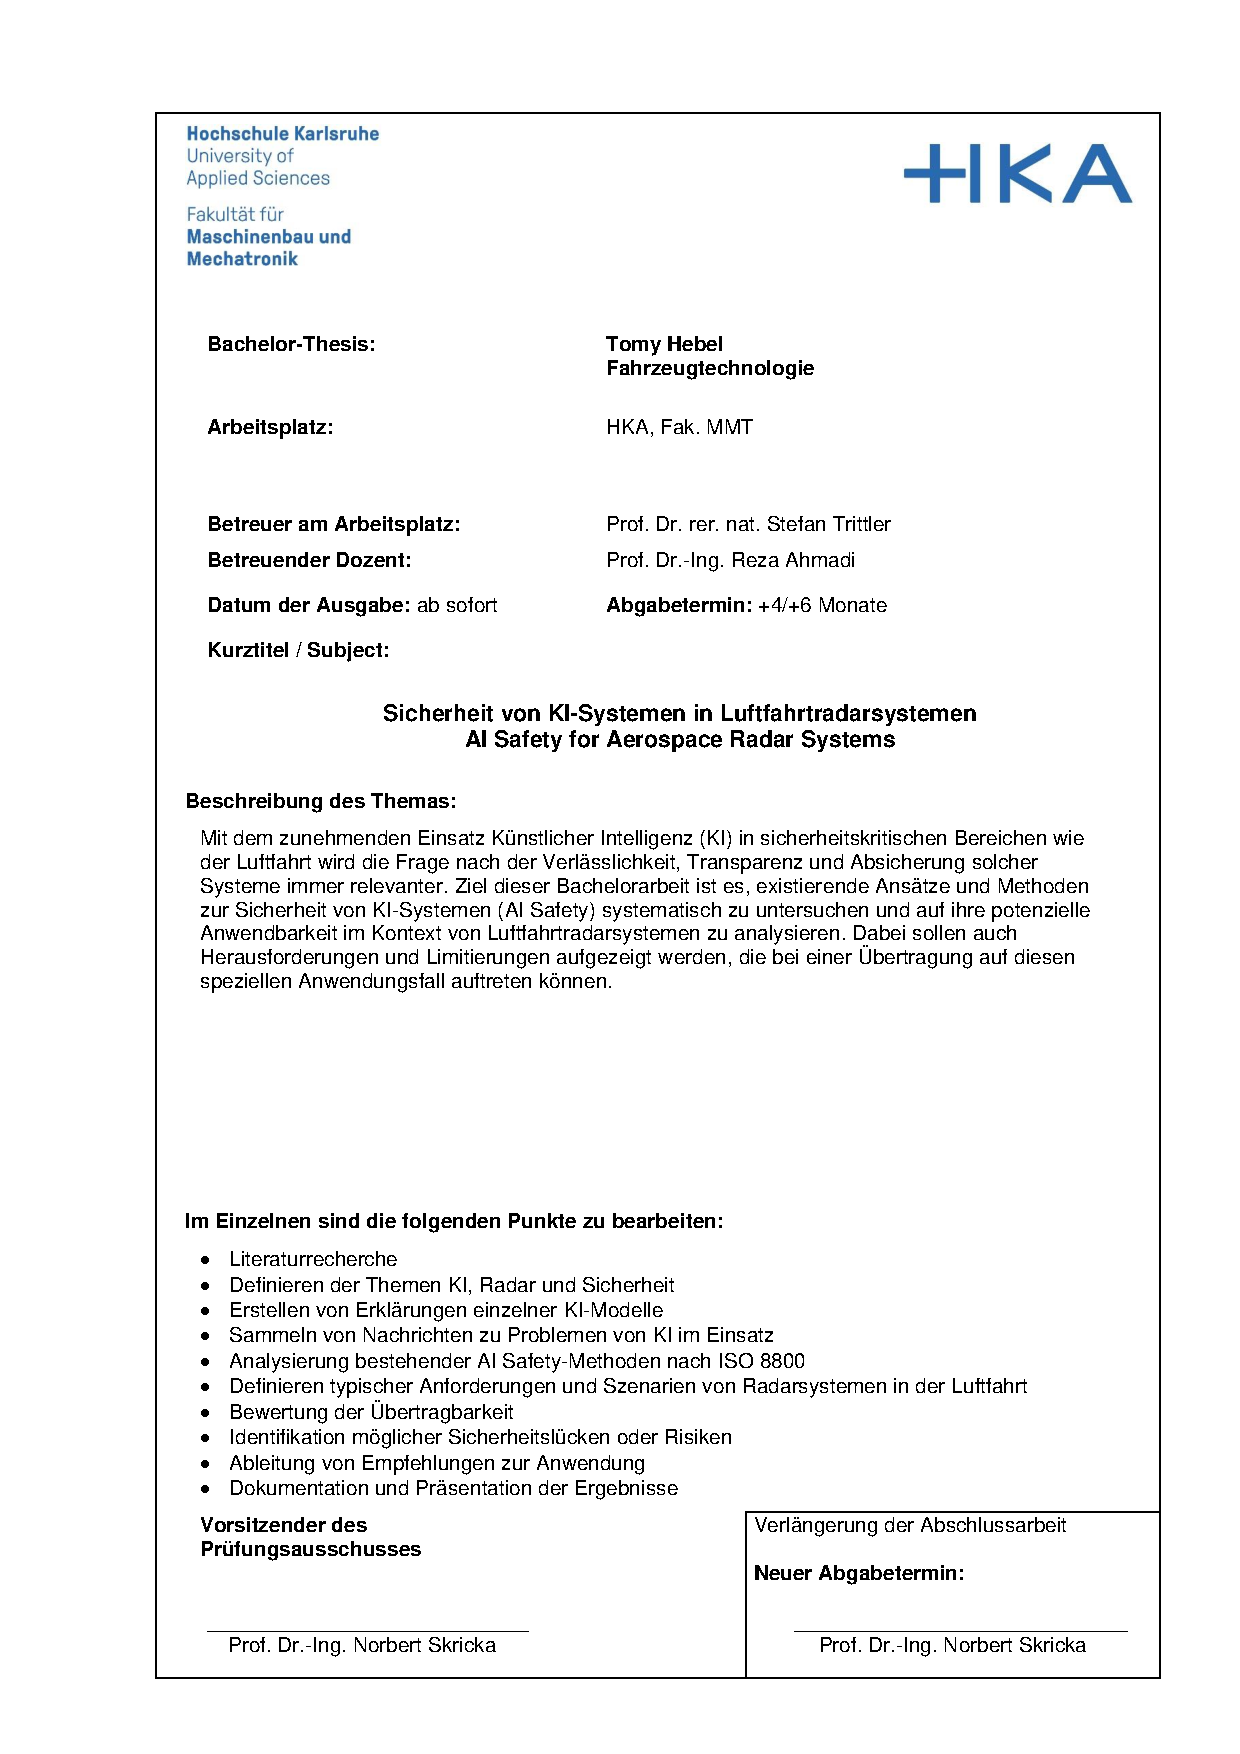
\includepdf[fitpaper=true, pages=-]{Bilder_und_Co/Sicherheit von KI-Systemen in Luftfahrtradarsystemen(1).pdf}

\chapter{Motivation und Ziel der Projektes}
Mit dem immer weiter verbreiteten Einsatz und Akzeptanz von \ac{KI} stellt sich die Frage, 
ob diese auch in der Luftfahrt Anwendung finden kann. Um diese Frage beantworten zu können, 
müssen \ac{KI} Modelle und ihr Eisatzgebiet auf Sicherheit überprüft werden. 

Ziel der Arbeit ist es, anhand des Beispieles von Radarsystemen zu überprüfen, 
ob KI-Systeme mittels bekannter Methodiken diese auf Sicherheit zu überprüfen ob sie den Anforderungen entsprechen, 
um diese in der Luftfahrt verwenden zu können.

\section{Weiteres}
In verschiedenen Paper wird gezeigt, dass \ac{KI} bei Radarsystemen was die Perfomance angeht, mit herkömmlichen Methoden 
mindestens mithalten kann oder diese was Rechenleistung, Speicher und Genauigkeit von Objekterkennung übertrifft. 
Dies unterstreicht weiter, dass es sehr nützlich sein kann \ac{KI} in diesem Feld zu benutzen. Doch in der Luftfahrt ist 
Sicherheit von großer Bedeutung und die meisten Paper die bei der Recherche zu diesem Thema gefunden wurden gehen 
auf die Performance der untersuchten KIs ein und untersuchen diese nicht auf Sicherheit, dies zeigt nochmals deutlich die Bedeutung 
dieser Arbeit. Doch was bedeutet sichere \ac{KI}? Ein Beispiel für eine Anforderung für eine sichere Software kann sein, 
dass diese deterministisch sein soll. Doch dies ist bezogen auf KIs problematisch umzusetzen, eine Möglichkeit wäre es, 
alle Möglichen Inputs und deren Outputs zu untersuchen bevor man die \ac{KI} verwendet. Aber das funktioniert nur bei 
kleieneren Modellen und würde vorallem bei Foundation Models einen zu großen Rechenaufwand bedeuten, als dass diese Methode 
verwendet werden könnte. Hier wäre eine persöhliche Idee einen Markowschen ansatz zu versuchen...??

\chapter{Hypothese}

\chapter{Methodisches Vorgehen}
\section{Besonders wichtige Literatur}
Zunächst wurde mit Absprache des Betreuenden Professors und dem Zweitkorrektor, eine kurze Liste an 
"Goldstandard-" Literatur festgelegt. Diese umfasst die recht neu erschienene ISO 8800 aus der Automobilbranche, 
welche die KI-Sicherheit in der Automobilbranche definiert. Die DO 178C weche über die Sicherheit von geschriebenen 
Computer Code in der Luftfahrt handelt. Und zum Schluss die EASA Roadmap und Concept Paper, welche beschreiben sollen, 
wie die Adaption von KI in der Luftfahrtbranche von statten gehen soll.


ISO 8800:

Diese ist die nach eigener Einschätzung, die derzeit Wertvollste Norm im Bezug auf KI-Sicherheit passend zum Kontext. 
Das liegt unteranderem an der Verwandschaft von der Luftfahrt und Automobilbranche, einerseitz technisch bzw. welche 
Ingenieurs-Fachgebiete abgedeckt werden, sowohl bei einem Flugzeug als auch bei einem Fahrzeug z.B. Aerodynamik, Elektrotechnik, 
Programmieren und vieles mehr. Die größeren Unterschiede hier liegen daher eher in den Anforderungen und Herangehensweisen 
im Bezug zur Sicherheit. Um beispielhafft einen sehr deutlichen Unterschied zu nennen, gibt es in der Automobilbranche 
die ISO 26262, die SOTIF Norm, welche sich mit der Sicherheit der Fuktionalität, unteranderem auch während des Betriebs 
des Fahrzeugs beschäftigt. Das kann zufolge haben, dass später im Lebenszyklus z.B. Softwareupdates erforderlich sind. 
Im Gegensatz wird in der Luftfahrt dieses Thema hauptsächlich im Frontloading behandelt, unter der Prämisse, dass das Flugzeug 
bereits bei erstigem Einsatz alle Sicherheitsanforderungen zur Gänze erfüllt und spätere Softwareupdates obsulet macht oder 
vorher definiert wird was und wann geändert werden muss mittels Updates.

Des Weiteren ähneln sich beide Branchen im Bezug auf die Sicherheit einzelner Komponenten. Z.B. werden in der Automobilbranche 
sehr hohe Sicherheitsanforderungen für einzelne Komponenten definiert, damit diese nicht redundant verbaut werden müssen und somit 
der Stückpreis pro Fahrzeug steigt, da bei Großserien redundante Teile sehr teuer sind. Hingegen wird in der Luftfahrt 
allgemein sehr hohe Ansprüche an alle einzelnen Teile gelegt, da die Gefahr bei Fehlfunktionen in einem Flugzeug sehr schnell 
lebensbedrohlich wird. Um weitere Sicherheit zu gewährleisten und um die definierten Anforderungen zu erfüllen werden die 
Teile in einem Flugzeug redundant verbaut.

Weitere Technische Unterschiede der Branchen gehen aus ihrer Natur herfor. In der Automobilbranche wird sehr viel B2C gehandelt, 
während die Luftfahrt hauptsächlich B2B handelt. Aufgrund der im Vergleich geringeren Lebensbedrohlichkeit bei Fehlfunktionen 
und der Branchennatur private Kunden zu gewinnen, befasst sich die Automobilbranche unteranderem viel mit technischen Begeisterungsmerkmahlen. 
Die Luftfahrt verfolgt das Ziel Geschäftskunden zu gewinnen, welche andere Wünsche haben als Privatpersonen.
Auf Grund dieses Unterschiedes kann sich die Automobilbranche sehr früh mit neueren Technologien auseinandersetzen, wo hingegen die 
Luftfahrt sich intensiv mit der Notwendigkeit und Sicherheit dieser neuen Technologien befasst. Weiter zu betrachten ist der gesammte Produktlebenszyklus, 
da Flugzeuge ca. zweimal so lange im Gebrauch sind wie Autos, was das Thema Sicherheit verkompliziert, besonders unter der Berücksichtigung 
von sich verändernde Umgebungen. (Beispiele hierfür sind im Straßenverkehr in den letzten Jahren eine größere Verbreitung von 
Elektrorollern zu beobachten. Und in der Luftfahrt nimmt der Einsatz von Dronen zu.)Z.B. kann die Automobilbranche mit einer KI 
gesteuerten Schilderkennung Kundengewinnen und Erfahrungen sammeln, während in der Luffahrt Wolken und Wetter Erkennung mit einer 
KI die Evaluierung und Entwicklung langwieriger ist. Das und noch mehr Gründe erklären, warum 
es die Luftfahrbranche daher technologisch träger macht. Aufgrund dieser Natur und der technischen Verwandheit wäre es sinnvoll, 
dass die Luftfahrt von den Erfahrungen der Automobilbranche lernen kann.


DO 178C:

Diese Luftfahrt Norm befasst sich mit der Sicherheit von geschrieben Computercode, zu erwähnen sind die Normen, auf die Bezug genommen werden in der 
DO 178C. Z.B. die DO 330 und die DO 333, welche sich mit Sofwarewerzeugen und deren Zertifizierung beschäftigen. Um den Aufwand nicht in das Unermessliche 
zu treiben werden diese nur bei bedarf angeschnitten. Da KI in verschiedener Literatur beschrieben "(z.b. ISO 5469TR)" als mathematischer 
Algorithmus und Teil der Softeware behandelt werden kann/sollte muss KI auch in Einklang gebracht werden mit der DO 178C. Was hier besonders interessant 
ist, sind bestimmte Anforderungen an Computer Code. Z.B. das der Code deterministisch sein soll und eine MC/DC coverage. Das KI oftmals nicht deterministisch 
ist, ist Allgemeinwissen. "(Unter bestimmten Vorraussetzungen kann KI deterministisch sein, z.B. wenn man die Temperatur des Outputvektors in einem NN auf 0 setzt 
und man den gesammten Inputraum abgedeckt/getestet hat. Doch das ist meistens technisch nicht umsetzbar oder würde die Funktion/Fähigkeit der KI zusehr einschränken)" 
MC/DC coverage beschreibt, dass jede einzelne Bedingung bei Entscheidungen z.B. if/else Schleifen im Code auch stehts ein anderen Output erzeugt. 
Das eine KI diese Anforderung nicht erfüllen kann sollte ebenfalls recht offensichtlich sein. Doch das interessante ist, dass in der 
DO 178C das nur implizit und nicht explizit gefordert wird. Um etwas genauer zu werden, werden diese Anforderungen sowohl in der DO 178C als auch 330 und 333 sehr 
empfohlen und als "best practise" beschrieben.


EASA AI Roadmap:

Die EASA ist die Europäische Agentur für Flugsicherheit. Die Regularien der EASA werden weltweit als "best practise" Standards anerkannt.
Und um Produkte in der europäischen Luftfahrtbranche anbieten zu können, müssen Flugzeughersteller EASA-Zulassungen besitzen. 
Auf Grund dieser Bedeutung und des Wissens und Erfahrungen der Sicherheitsingenieure dieser Agentur, muss nicht weiter 
ausgeführt werden, warum diese veröffentlichten Konzepte hier mit besonderer Bedeutung berücksichtigt wurden.
Doch leider sind die Veröffentlichten Konzepte leider nicht mehr als genau das. In diesen Konzepten stehen 
viele "best practise" Methoden und zu berücksichtigende Punkte, jedoch leider nicht, wie bei einer Norm, 
dass wenn alle dieser Punkte erfüllt sind, dass das Produkt sicher ist. Hier ein kleiner Spoiler vorab, sehr viele dieser Punkte 
und Methoden sind deckungsgleich mit dem was in der ISO 8800 steht. Die ISO 8800 geht konkreter auf Anpassungen 
zu berücksichtigender Normen ein und beschreibt ins Detail was wie Dokumentiert werden muss. "(Weiteres später)"

\section{Recherche}
Der zweite Schritt war weitere Literaturrecherche. Für die vorliegende Recherche wurden verschiedene wissenschaftliche Quellen systematisch ausgewertet. 
Dabei kamen unter anderem etablierte Datenbanken wie Google Scholar, ProQuest und IEEE Xplore zum Einsatz. 
Zur Sicherstellung einer umfassenden Betrachtung des Themas wurde die Auswahl der Quellen jedoch nicht 
ausschließlich auf diese Datenbanken beschränkt, sondern durch weitere spezialisierte Plattformen und 
einschlägige Fachpublikationen ergänzt. Ziel war es, eine breite und ausgewogene Grundlage für die Analyse 
und Darstellung der Thematik zu schaffen. Zudem war das Vorgehen zuerst anhand des Titels eine Thematische 
Verwandschaft festzustellen. Wenn im Titel kein Hinweis auf eines der Subthemen: KI, Radarsysteme, Luftfahrt 
oder Sicherheit zu erkennen war, wurden die Wissenschaftlichen Paper nicht weiter evaluiert. Die Paper, 
die ein Hinweis auf mindestens eines dieser Subthemen aufwieß wurde es Systematisch festgehalten und anhand 
des Abstractes auf tiefergehende Relevanz untersucht. Wenn das Abstract weitere Thematische Zusammenhänge 
gezeigt hat, wurde es berücksichtigt. Probleme die hier öfter aufgetreten sind waren, dass im Kontext KI 
es sich oftmals um Performance Paper gehandelt hat. Diese Performance Paper folgten meist dem Schema zu erklären, 
wie, warum und wofür diese KI trainiert wurde und ihre Fähigkeiten aufgezeigt. Diese Paper hatten zwei Probleme, 
einerseits waren sie nicht besonders relevant für das Thema und eine relative Performance im Vergleich zu 
herkömmlichen Methoden wurde meist auch nicht ausgeführt.


\chapter{Aufbau der Arbeit} 
\part{Radar in der Luftfahrt}
\chapterimage{Bilder_und_Co/a_magnifying_glass_which_points_out_a_neuronal_network_surrounded_by_computer_code_and_a_question_ma_296098326.png} % Chapter heading image
%----------------------------------------------------------------------------------------
\chapter{Radar Grundlagen}

\section{Prinzip}
Senden–Empfangen von EM-Wellen, 
Laufzeit => Entfernung, 
Doppler => Relativgeschwindigkeit, 
Antenne/Beam => Winkel.

\section{Wichtige Größen}
SNR, PRF, Pulsbreite, 
Bandbreite/Entfernungsauflösung, 
Dopplerauflösung, Beamwidth, 
CFAR (Konstante Falschalarmrate).

\section{Datenformen}
I/Q-Daten → Range-Doppler-Map (RD) → 
ggf. Range-Doppler-Angle (RDA) → Detektionen/Tracks.

\section{Leistungskennzahlen}
Entdeckungswahrscheinlichkeit Pd, Falschalarmrate Pfa, 
Reichweite, Aktualisierungsrate, Latenz.

\section{Limits und Störer}
Clutter (Boden/Meer/Wetter), Mehrwege, RFI, 
Abschattung, Ambiguitäten (Range/Doppler).



\chapter{Radar im Luftfahrtkontext}

\section{Bodenradar}
Primärradar (PSR), 
Sekundärradar (SSR/Mode A/C/S), 
Multilateration/ADS-B (kooperativ).

\section{Bordradar}
Wetterradar (WXR), 
Kollisionsvermeidung/TAWS-Umfeld, 
Hinderniserkennung.

\section{Typischer Signalpfad}
Rohdaten → Pulskompression/FFT → CFAR → Clustering → Tracking → HMI.

\section{Leistungsanforderungen}
Abdeckung von Terminal/En-Route, Track-Kontinuität, 
Koexistenz mit ADS-B/TCAS, Verfügbarkeit/Redundanz.


\chapter{Wichtiges mitzunehmen}
\section{Merksatz}
Gute Klassifikation ist nur so gut wie die Stabilität von RD/RDA und der Track-Qualität. 
\part{Sicherheit in der Luftfahrt}
\chapterimage{Bilder_und_Co/a_radar_system_at_an_airport_tower_1403000730.png} % Chapter heading image
%----------------------------------------------------------------------------------------
\chapter{Sicherheit Grundlagen} 

\section{Safety vs. Security}
Unbeabsichtigte Fehler vs. absichtliche Angriffe.

\section{Risikobegriff}
Schweregrad × Eintrittswahrscheinlichkeit; fail-safe vs. fail-operational.

\section{Methoden}
Hazard-Analyse (FHA), FMEA/FMECA, Fault-Tree, Bow-Tie; „Defense in Depth“.

\section{Prozesse}
Anforderungen → Architektur → Verifikation/Validierung → Betrieb/Änderungsmanagement.



\chapter{Luftfahrt-spezifische Sicherheit} 

\section{Safety-Entwicklung}
ARP4754A (System), ARP4761 (Safety), DO-178C (Software), DO-254 (Hardware).

\section{Assurance Level}
DAL A–E je nach Kritikalität (z. B. Kollision vermeiden => hoch).

\section{Security-Framework}
DO-326A/356A/355A (Airworthiness Security, Methoden, Betrieb).

\section{Betrieb}
Continuing Airworthiness, Konfigurationskontrolle, Audits, Incident-Response.

\section{Metriken und Evidenz}
Nachweisbarkeit, Rückverfolgbarkeit (Requirements <-> Tests), Abdeckungsgrade.




\chapter{Wichtiges mitzunehmen}
\section{Merksatz}
In der Luftfahrt zählt nicht nur „funktioniert“, sondern „ist nachweislich sicher und beherrschbar“.
\part{KI in der Luftfahrt}
\chapterimage{Bilder_und_Co/a_radar_system_at_an_airport_tower_1403000730.png} % Chapter heading image
%----------------------------------------------------------------------------------------
\chapter{Use-Cases} 
\part{KI Sicherheit}
\chapterimage{Bilder_und_Co/a_radar_system_at_an_airport_tower_1403000730.png} % Chapter heading image
%----------------------------------------------------------------------------------------
\chapter{Begriffe} 

\section{AI Safety}
= beherrschbares, verlässliches Verhalten (funktionale Sicherheit, Fehlertoleranz).

\section{AI Security}
= Schutz der KI vor Angriffen (Poisoning, Adversarial, Model Theft).

\section{Airworthiness Security}
= luftfahrtspezifische Security-Prozesse.




\chapter{Risiken}
Safety-Fehler (Fehlklassifikation, schlechte Kalibrierung, OOD-Blindheit) 
vs. Security-Angriffe (Jamming/DRFM auf Sensor-Ebene, Backdoors/Adversarial auf ML-Ebene).

\chapter{Design-Prinzipien}
\section{Safety}
Kalibrierung, Unsicherheits-Schätzung, Abstain/Unknown, Safety-Cage/Simplex, erklärbare Features.

\section{Security}
Daten-Governance, signierte Modelle/secure boot, OOD/Anomalie-Wächter, adversarial Training, Red-Team-Tests.

\chapter{Metriken und Evidenz}
ECE/Brier, OOD-Rate, adversarial Erfolgsrate, J/S-Robustheit, Traceability (Req <-> Test <-> Befund).
\part{KI in Radarsystemen}
\chapterimage{Bilder_und_Co/safety_sign_with_computer_code_and_a_airplane_in_the_background_1958542794.png} % Chapter heading image
%----------------------------------------------------------------------------------------
\chapter{KI Grundlagen}

\section{Begriffe}
ML vs. DL, überwachtes/teil-/unüberwachtes Lernen, Features vs. End-to-End.

\section{Datenpraxis}
Train/Valid/Test, saubere Splits (keine Leckagen), Domain Shift, Augmentation.

\section{Bewertung}
Precision/Recall/F1 pro Klasse, ROC/PR, Kalibrierung (ECE/Brier), Latenz/Throughput.

\section{Verlässlichkeit}
Unsicherheitsabschätzung, OOD-Erkennung, „Abstain/Unknown“, Erklärbarkeit (Saliency/Prototypen).

\section{Fehlermodi}
Overfitting, Datenbias, Verteilungsdrift, Spurious Correlations.




\chapter{KI im Radar}

\section{Einsatzfelder}
Clutter-Unterdrückung, Detektion, Objektklassifikation (z. B. Flugzeug/Heli/UAS/Vogel), 
Tracking/Track-Fusion, Ressourcen-Management (Waveform Scheduling).

\section{Eingaben}
RD/RDA-Tensors, Mikro-Doppler-Spektrogramme, Track-Sequenzen; 
physikgeleitete Features (RCS, Spektralbreite, Manöver).

\section{Modelle}
2D/3D-CNN/ViT (bildartig), LSTM/TCN/Transformer (zeitlich), hybride physik-informierte Netze.

\section{Runtime und Architektur}
Latenzbudgets, Quantisierung/Pruning für FPGA/SoC, Safety-Cage/Simplex als Fallback.

\section{Security-Basics}
Adversarial Examples (RD-Domäne), Data-Poisoning/Backdoors, Model-Stealing; 
harte vs. weiche Abwehrmaßnahmen.




\chapter{Wichtiges mitzunehmen}
\section{Merksatz}
In sicherheitskritischen Radaranwendungen ist KI kalibriert, OOD-fähig und in eine sichere Runtime-Architektur eingebettet.



%
%----------------------------------------------------------------------------------------
%	Part 2: Format Examples (to be deleted in final/release version)
\part{TEIL 2}
%----------------------------------------------------------------------------------------

\chapterimage{Pictures/csm_HKA_FK-MMT_Imagefoto_9847_0f123dde52.jpg} % Chapter heading image

\chapter{Formatierungen und Templates}

\section{Table}\index{Table}

\begin{table}[h]
\centering
\begin{tabular}{l l l}
\toprule
\textbf{Treatments} & \textbf{Response 1} & \textbf{Response 2}\\
\midrule
Treatment 1 & 0.0003262 & 0.562 \\
Treatment 2 & 0.0015681 & 0.910 \\
Treatment 3 & 0.0009271 & 0.296 \\
\bottomrule
\end{tabular}
\caption{Table caption}
\label{tab:example} % Unique label used for referencing the table in-text
%\addcontentsline{toc}{table}{Table \ref{tab:example}} % Uncomment to add the table to the table of contents
\end{table}

Referencing Table \ref{tab:example} in-text automatically.


%------------------------------------------------
\section{Citation}\index{Citation}

This statement requires citation \cite{article_key}; this one is more specific \cite[162]{book_key}.

%------------------------------------------------

\section{Lists}\index{Lists}

Lists are useful to present information in a concise and/or ordered way\footnote{Footnote example...}.

\subsection{Numbered List}\index{Lists!Numbered List}

\begin{enumerate}
\item The first item
\item The second item
\item The third item
\end{enumerate}

\subsection{Bullet Points}\index{Lists!Bullet Points}

\begin{itemize}
\item The first item
\item The second item
\item The third item
\end{itemize}

\subsection{Descriptions and Definitions}\index{Lists!Descriptions and Definitions}

\begin{description}
\item[Name] Description
\item[Word] Definition
\item[Comment] Elaboration
\end{description}

This is an example of theorems.

\subsection{Several equations}\index{Theorems!Several Equations}
This is a theorem consisting of several equations.

\begin{theorem}[Name of the theorem]
In $E=\mathbb{R}^n$ all norms are equivalent. It has the properties:
\begin{align}
& \big| ||\mathbf{x}|| - ||\mathbf{y}|| \big|\leq || \mathbf{x}- \mathbf{y}||\\
&  ||\sum_{i=1}^n\mathbf{x}_i||\leq \sum_{i=1}^n||\mathbf{x}_i||\quad\text{where $n$ is a finite integer}
\end{align}
\end{theorem}

\subsection{Single Line}\index{Theorems!Single Line}
This is a theorem consisting of just one line.

\begin{theorem}
A set $\mathcal{D}(G)$ in dense in $L^2(G)$, $|\cdot|_0$. 
\end{theorem}

%------------------------------------------------

\section{Definitions}\index{Definitions}

This is an example of a definition. A definition could be mathematical or it could define a concept.

\begin{definition}[Definition name]
Given a vector space $E$, a norm on $E$ is an application, denoted $||\cdot||$, $E$ in $\mathbb{R}^+=[0,+\infty[$ such that:
\begin{align}
& ||\mathbf{x}||=0\ \Rightarrow\ \mathbf{x}=\mathbf{0}\\
& ||\lambda \mathbf{x}||=|\lambda|\cdot ||\mathbf{x}||\\
& ||\mathbf{x}+\mathbf{y}||\leq ||\mathbf{x}||+||\mathbf{y}||
\end{align}
\end{definition}

%------------------------------------------------

\section{Notations}\index{Notations}

\begin{notation}
Given an open subset $G$ of $\mathbb{R}^n$, the set of functions $\varphi$ are:
\begin{enumerate}
\item Bounded support $G$;
\item Infinitely differentiable;
\end{enumerate}
a vector space is denoted by $\mathcal{D}(G)$. 
\end{notation}

%------------------------------------------------

\section{Remarks}\index{Remarks}

This is an example of a remark.

\begin{remark}
The concepts presented here are now in conventional employment in mathematics. Vector spaces are taken over the field $\mathbb{K}=\mathbb{R}$, however, established properties are easily extended to $\mathbb{K}=\mathbb{C}$.
\end{remark}

%------------------------------------------------

\section{Corollaries}\index{Corollaries}

This is an example of a corollary.

\begin{corollary}[Corollary name]
The concepts presented here are now in conventional employment in mathematics. Vector spaces are taken over the field $\mathbb{K}=\mathbb{R}$, however, established properties are easily extended to $\mathbb{K}=\mathbb{C}$.
\end{corollary}

%------------------------------------------------

\section{Propositions}\index{Propositions}

This is an example of propositions.

\subsection{Several equations}\index{Propositions!Several Equations}

\begin{proposition}[Proposition name]
It has the properties:
\begin{align}
& \big| ||\mathbf{x}|| - ||\mathbf{y}|| \big|\leq || \mathbf{x}- \mathbf{y}||\\
&  ||\sum_{i=1}^n\mathbf{x}_i||\leq \sum_{i=1}^n||\mathbf{x}_i||\quad\text{where $n$ is a finite integer}
\end{align}
\end{proposition}

\subsection{Single Line}\index{Propositions!Single Line}

\begin{proposition} 
Let $f,g\in L^2(G)$; if $\forall \varphi\in\mathcal{D}(G)$, $(f,\varphi)_0=(g,\varphi)_0$ then $f = g$. 
\end{proposition}

%------------------------------------------------

\section{Examples}\index{Examples}

This is an example of examples.

\subsection{Equation and Text}\index{Examples!Equation and Text}

\begin{example}
Let $G=\{x\in\mathbb{R}^2:|x|<3\}$ and denoted by: $x^0=(1,1)$; consider the function:
\begin{equation}
f(x)=\left\{\begin{aligned} & \mathrm{e}^{|x|} & & \text{si $|x-x^0|\leq 1/2$}\\
& 0 & & \text{si $|x-x^0|> 1/2$}\end{aligned}\right.
\end{equation}
The function $f$ has bounded support, we can take $A=\{x\in\mathbb{R}^2:|x-x^0|\leq 1/2+\epsilon\}$ for all $\epsilon\in\intoo{0}{5/2-\sqrt{2}}$.
\end{example}

\subsection{Paragraph of Text}\index{Examples!Paragraph of Text}

\begin{example}[Example name]
\lipsum[2]
\end{example}

%------------------------------------------------

\section{Exercises}\index{Exercises}

This is an example of an exercise.

\begin{exercise}
This is a good place to ask a question to test learning progress or further cement ideas into students' minds.
\end{exercise}

%------------------------------------------------

\section{Problems}\index{Problems}

\begin{problem}
What is the average airspeed velocity of an unladen swallow?
\end{problem}

%------------------------------------------------

\section{Vocabulary}\index{Vocabulary}

Define a word to improve a students' vocabulary.

\begin{vocabulary}[Word]
Definition of word.
\end{vocabulary}


%------------------------------------------------

\section{Figure}\index{Figure}

\begin{figure}[h]
\centering\includegraphics[scale=0.5]{Pictures/placeholder.jpg}
\caption{Figure caption}
\label{fig:placeholder} % Unique label used for referencing the figure in-text
%\addcontentsline{toc}{figure}{Figure \ref{fig:placeholder}} % Uncomment to add the figure to the table of contents
\end{figure}

Referencing Figure \ref{fig:placeholder} in-text automatically.	% TODO: uncomment for final version!


%----------------------------------------------------------------------------------------
%	BIBLIOGRAPHY
%----------------------------------------------------------------------------------------
\cleardoublepage
\part*{Bibliography}
\chapterimage{Bilder_und_Co/bibliography_3467130032.png} % Chapter heading image
\chapter*{Bibliography}
\addcontentsline{toc}{chapter}{\textcolor{ThemeColor}{Bibliography}} % Add a Bibliography heading to the table of contents
\fancyhead[LE,LO]{\sffamily\normalsize\thepage} % Header - Odd-Even Page - Left side - show page numbers 
\fancyhead[RE,RO]{\textbf \bibname} % Header - Odd-Even Page - Right side - show Bibliography text
\printbibliography[heading=bibempty]

%----------------------------------------------------------------------------------------
%	INDEX
%----------------------------------------------------------------------------------------

%\cleardoublepage % Make sure the index starts on an odd (right side) page
%\phantomsection
%\setlength{\columnsep}{0.75cm} % Space between the 2 columns of the index
%\addcontentsline{toc}{chapter}{\textcolor{ThemeColor}{Index}} % Add an Index heading to the table of contents
%\printindex % Output the index

%----------------------------------------------------------------------------------------

\end{document}
